\section{Organisation de l'équipe}
\paragraph{Jusqu'à maintenant, la plupart des projets que nous avions eu à faire à l'Imac se déroulaient par binôme ou au maximum trinôme. Dans ces cas-là, la gestion du groupe s'en trouvait simplifiée car la répartition du travail était simple. Dans le cas d'une équipe de six personnes, il est nécessaire de bien connaître les aptitudes, les passions et motivations de chaque membre pour en tirer le maximum pour le bien de l'équipe (\textit{plus on aime ce que l'on fait, plus on le fait bien}). De plus, nous avons eu la chance - légèrement provoquée - que chaque membre de notre équipe provient de filières très différentes et possède des connaissances et talents très complémentaires.}

\paragraph{Un projet de programmation comme Smashstein demande en effet beaucoup de connaissances et de travail dans ce domaine, c'est pourquoi la grande majorité de l'équipe s'est attelée à cette tâche à un moment ou à un autre de l'avancement. Cependant, la programmation est à un projet comme Smashstein le ciment est à un bâtiment, il est nécessaire de créer de l'enrobage et de la matière autour pour lui donner une forme plus esthétique et agréable. C'est dans cet optique que nous avons concentré la seconde partie de l'équipe dans la réalisation des éléments graphiques tel que les modèles 3D ou les décors. Un jeu sans attrait graphique peut vite perdre de son intérêt. Le dernier membre de l'équipe s'est entièrement dédié à l'univers sonore car cette fonction est bien souvent mise en défaut alors que sans elle, un jeu peut bien vite sembler fade et triste.}

\paragraph{Ainsi, nous avons su trouver dans cette équipe toutes les compétences nécessaires au bon déroulement de ce projet afin qu'il aboutisse de la meilleure des façons malgré le peu de temps qui nous était imparti.}

\newpage
\section{\'Etablissement du planning}


\subsection{Planning prévisionnel}
\vspace{0.5cm}

\paragraph{Avant de démarrer le projet, il nous a semblé nécessaire de nous réunir afin de partager nos idées. Les phases de réflexion ne sont évidemment pas à négliger, puisque c'est le tremplin pour partir d'une m\^eme base. Nous savions par la suite ce qui devrait \^etre plus ou moins fait. Autrement dit, nous nous sommes répartis les t\^aches selon nos affinités avec tel ou tel domaine. C'est ainsi qu'un rétroplanning a été aussit\^ot mis en place. Ce planning prévisionnel permet de fixer quelques dates clés, d'avoir une vue d'ensemble des t\^aches à effectuer et d'avoir un repère dans la progression de ce projet.}
\vspace{0.5cm}
\hspace{-2cm}
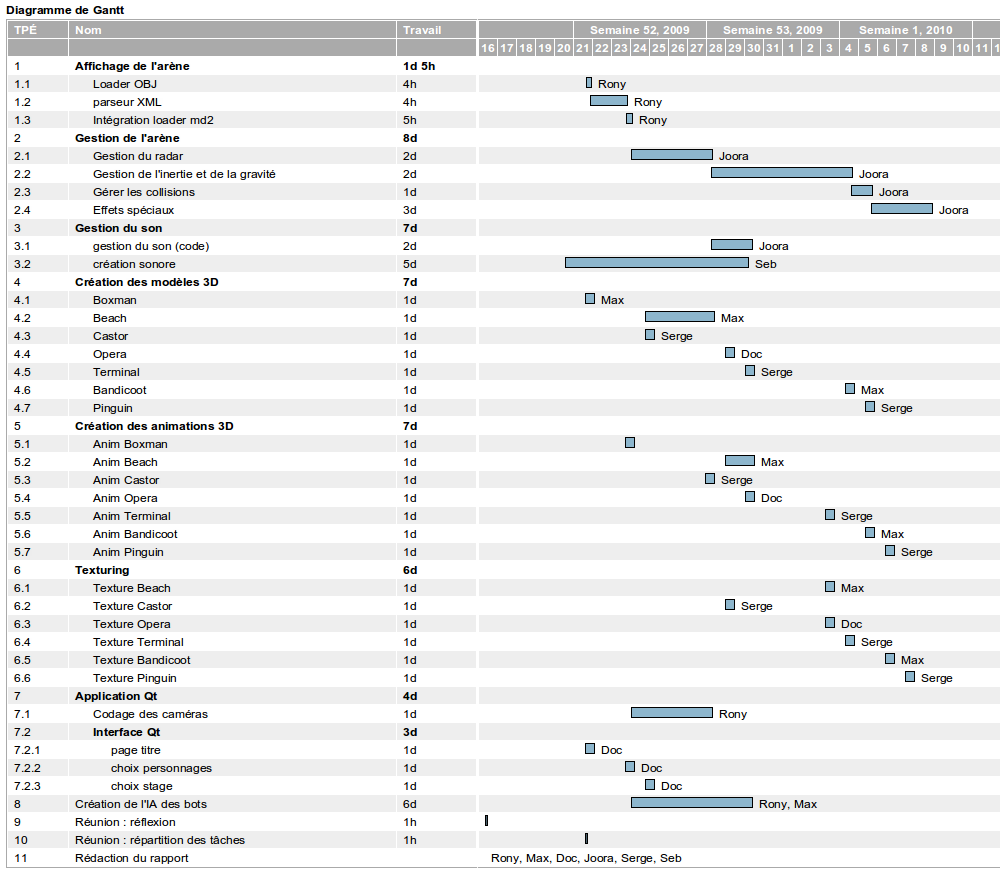
\includegraphics[scale=0.5]{visuel/retroplanning.png}
\hspace{0cm}

\subsection{Planning réel}
\vspace{1cm}

\paragraph{Après quelques semaines de travail, le planning réel a été dressé. Ce qui est intéressant, c'est de constater les changements par rapport au planning initial. Par exemple, nous avons mis en retrait la modélisation et animation de quelques personnages. Ou encore, certaines t\^aches ont pris plus de temps que prévu. Les f\^etes de fin d'année y sont probablement pour quelques choses.}

\hspace{-1cm}
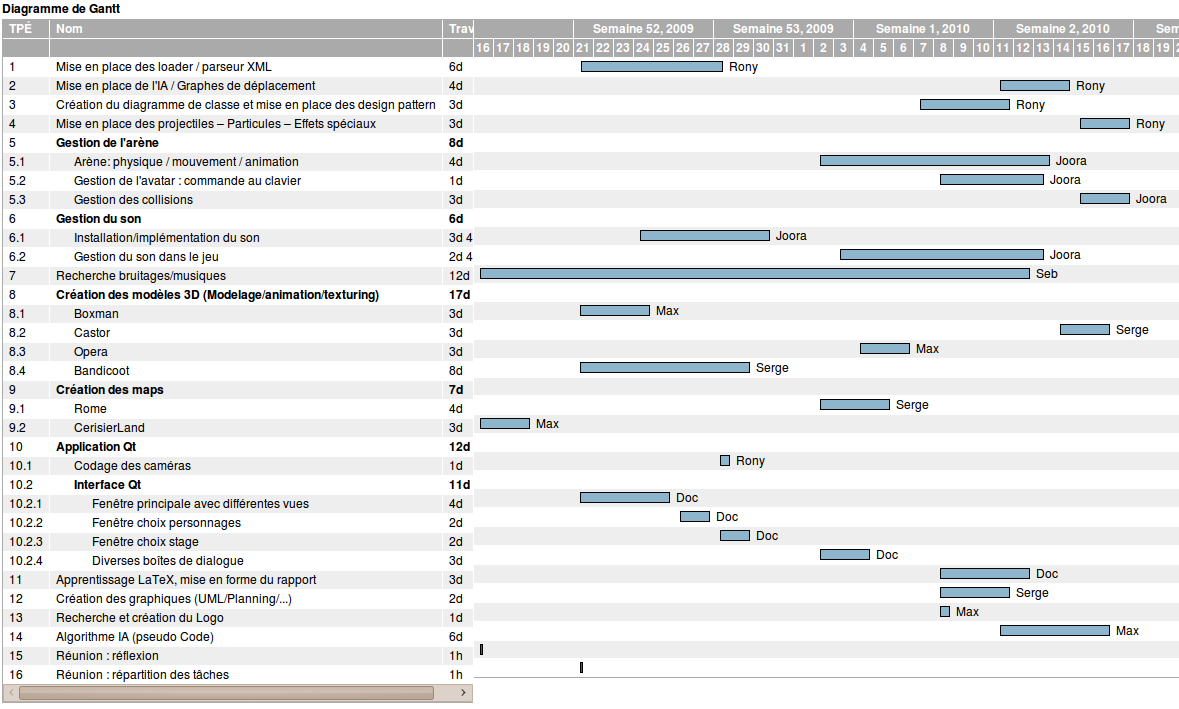
\includegraphics[scale=0.4]{visuel/planning-reel.png}
\hspace{0cm}

\newpage
\section{Organisation du travail}
\subsection{Mise en place de quelques conventions}
\vspace{0.5cm}

\paragraph{Avant de se lancer dans la programmation du jeu, nous nous sommes mis d'accord sur la façon de présenter le code. En effet, la mise en place de quelques règles d'écriture était nécessaire. Ceci permet d'avoir un code cohérent mais surtout plus compréhensible par tous les membres du groupe et donc plus facilement maintenable.}
\paragraph{Voici ces quelques règles :}

\begin{itemize}
	\item Le nom des classes, méthodes, attributs, variables, fonctions... en anglais 
	\item Le nom des classes commencent par une majuscule
	\item Les autres noms commencent par une minuscule et le mot composé qui suit par une majuscule
	\item Les accolades des blocs d'instructions sont alignées verticalement :
	\begin{verbatim}
		void method()
		{
		    ...		
		}
	\end{verbatim}
\end{itemize}


\vspace{1cm}
\subsection{Outil de travail collaboratif}
\vspace{0.5cm}

\paragraph{Deux outils de travail ont été mis en place dès le départ afin de faciliter la communication entre nous et la coordination des travaux réalisés :}

\begin{itemize}
	\item une liste de diffusion privée
	\item un système de gestion de versions
\end{itemize}

\vspace{0.5cm}

\paragraph{Tous les échanges de courriers électroniques se sont fait à travers cette adresse de diffusion : \verb?list-smashtein@pandaco.net?. \'Etant donné que nous n'étions que six dans cette liste, nous nous sommes permis de l'utiliser sans retenue. Ainsi, quelque soit la discussion, tous les membres se tenaient au courant.}

\paragraph{Concernant le choix du système de versionning, nous avons opté de mettre en place un dép\^ot centralisé de type Subversion. Nous l'avons déjà utilisé par le passé, nous étions donc plus ou moins aisés face à cet outil bien pratique. De ce fait, tous nos travaux étaient constamment synchronisés avec le dép\^ot. Afin d'éviter les conflits, nous nous mettons toujours d'accord sur quelles parties nous allons travailler.}

\newpage
\section{Architecture logicielle}
\vspace{0.5cm}
\paragraph{Dans l'optique de ce projet, nous avons décidé de réaliser un diagramme de classe qui répondrait aux principales fonctionnalités du programme de la façon la plus idéale possible. Pour ce faire, nous avons utilisé différents design patterns pour répondre à des situations bien précises. Nous n'allons bien s\^ur pas décrire la totalité de nos choix pour ce diagramme de classe dans ce rapport. Cela serait inutile et redondant. Cependant, nous expliciterons tout de même nos choix en ce qui concerne les principaux design pattern mis en place.}

\paragraph{L'arène dans ce projet est l'élément central. C'est un objet unique et nous utilisons le design pattern « \textbf{Singleton} » pour le représenter. Elle utilise une \textbf{Factory} via la classe \textit{Robots} pour générer les bots qui bénéficient d'une IA\footnote{Intelligence Artificielle} et l'avatar contrôlé par le personnage.}

\paragraph{L'arène utilise une \textit{Collection} pour stocker les objets 3D chargés via les .OBJ\footnote{Voir Section 3.6.1}. Elle gère deux collections : les objets du décor non-interactif \textit{DecorMesh} et les objets interactifs qui rentrent dans la gestion des collisions \textit{IOMesh}. Bien entendu, il existe des itérateurs pour parcourir ces différents objets dans les collections.}

\paragraph{L'arène et les bots qui possèdent une IA répondent au design pattern \textbf{Observateur}. En effet, chaque robot peut s'abonner à l'arène qui lui indique à partir de quel moment il peut effectuer une nouvelle action et lui communique les ennemis qui l'ont frappés...}

\paragraph{Une fois un bot créé, il faut être capable de lui attribuer certaines caractéristiques tel que son modèle md2, ses animations, ou encore son intelligence artificielle. Dans deux de ces cas, nous utilisons un autre design pattern pour les mettre en place. Le design pattern \textbf{Strategy} a été utilisé. L'interface \textit{Movement} en effet, permet de gérer toutes les animations du modèle 3d (run, jump, attack...) et l'interface \textit{Brain} gère, quant à elle, les « cerveaux » du bot pour pouvoir modifier dynamiquement les comportements qui vont influencer les actions du robot dirigé par l'ordinateur.}
	
\paragraph{Dans de nombreux autres cas, nous avons mis en place des interfaces qui vont faciliter la gestion des classes et des objets. Tels que tous les objets interactifs sont des obstacles. L'interface projectile pour gérer les projectiles de l'arène.}

\paragraph{Chaque \textit{Robot} implémente l'interface robot et possède des éléments tels que leur \textit{speakers} qui implémentent, eux aussi, d'autres interfaces. Nous nous sommes efforcés de mettre tout ce qui nous paraissait commun en interface afin de faciliter la gestion et la compréhension du programme.}



\newpage
\subsection{Diagramme de classe - première partie}
\vspace{0.5cm}
\hspace{-1.5cm}
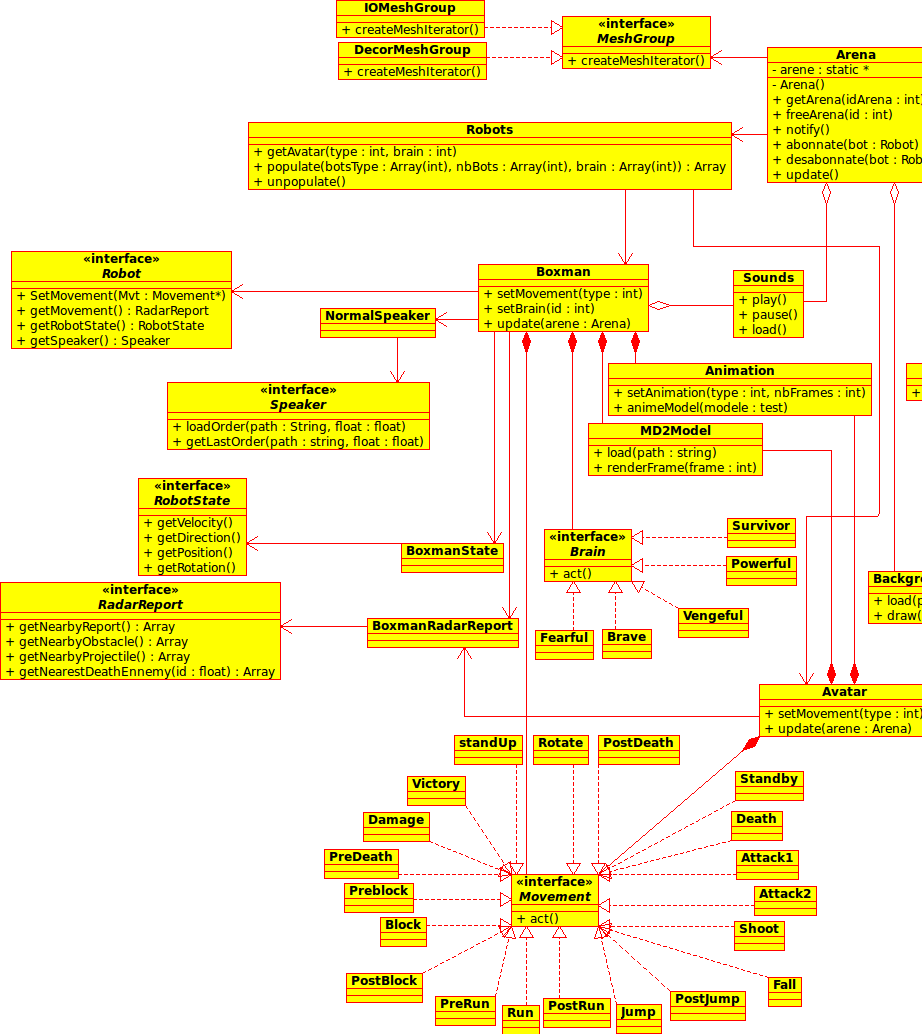
\includegraphics[scale=0.7]{visuel/uml-diagramme-classe-part1.png}

\newpage
\hspace{0cm}
\subsection{Diagramme de classe - seconde partie}
\vspace{0.5cm}
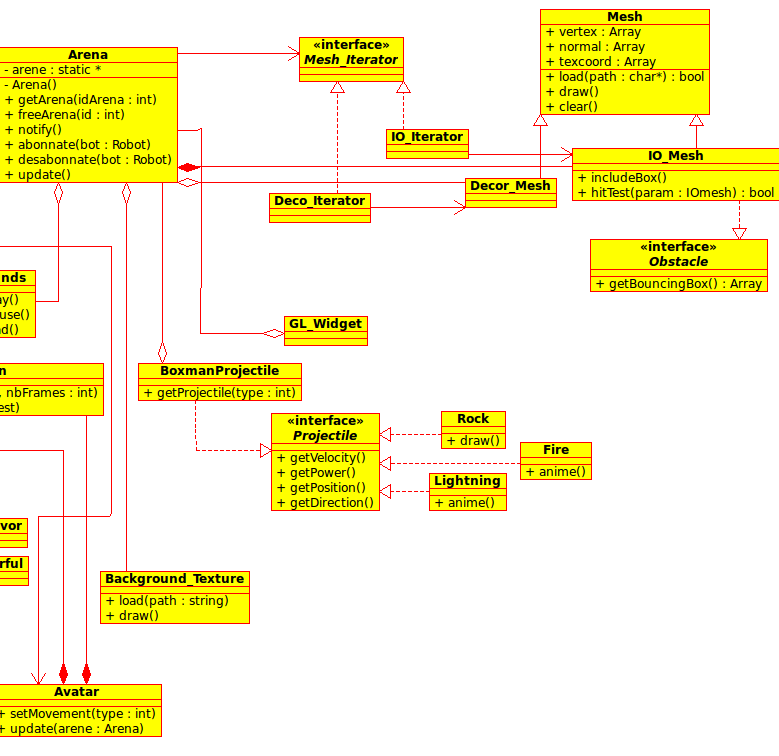
\includegraphics[scale=0.7]{visuel/uml-diagramme-classe-part2.png}
